\documentclass[xcolor=table, 10pt, aspectratio=169]{beamer}

%\usepackage{arev}
\usepackage{amsmath,amssymb,amscd}
\usepackage{dsfont}
\usepackage{mathrsfs}
\usepackage{yfonts}
\usepackage{bm}
\usepackage{graphicx}
\usepackage{tabularx}
\usepackage{animate}
%\usepackage{mathtools}
%\usepackage{ifthen}

%\usepackage{xeCJK}
%\usepackage{fontspec}
%\newfontfamily\cjkfont{PingFang SC}
%\setCJKmainfont{PingFang SC}
\newcolumntype{x}{>{\centering\arraybackslash}X}
\renewcommand{\arraystretch}{1.5}

\usepackage{tikz}
	\usetikzlibrary{calc}
	\usetikzlibrary{arrows,shapes, positioning, matrix}
	\usetikzlibrary{decorations.markings}
	\tikzset{>=stealth}
	\tikzstyle arrowstyle=[scale=1]
	\tikzstyle directed=[postaction={decorate,decoration={markings,
 	   mark=at position .15 with {\arrow[arrowstyle]{stealth}}}}]
\tikzstyle string=[thick,postaction={decorate,decoration={markings,
    mark=at position .55 with {\arrow[arrowstyle]{stealth}}}}]
\tikzstyle dual_string=[dashed,postaction={decorate,decoration={markings,
    mark=at position .55 with {\arrow[arrowstyle]{stealth}}}}]

\tikzstyle dw=[thick,postaction={decorate,decoration={markings,
    mark=at position 1 with {\arrow[arrowstyle]{stealth}}}}]
\tikzstyle group=[mbg]
\newcommand*{\halfway}{0.5*\pgfdecoratedpathlength+.5*8pt}\tikzstyle arrowstyle=[scale=1]
\newcommand*{\halfwayb}{0.5*\pgfdecoratedpathlength}
\tikzstyle arrowstyle=[scale=1]
\tikzstyle fermion=[thick,postaction={decorate},decoration={markings,
    mark=at position \halfway with {\arrow[arrowstyle]{latex}}}]
\tikzstyle fermion2=[thick,postaction={decorate},decoration={markings,
        mark=at position \halfwayb with {\arrow[arrowstyle]{latex}}}]

\usepackage{pgffor}
\newcommand{\mb}[1]{\mathbf{#1}}
\renewcommand{\cal}[1]{\mathcal{#1}}

\newcommand{\ag}[2]{#1_\mb{#2}}
\newcommand{\cohosub}[1]{\scalebox{0.72}{\textswab{#1}}}
\newcommand{\cohosubsub}[1]{\scalebox{0.6}{\textswab{#1}}}
\newcommand{\coho}[1]{\textswab{#1}}

\DeclareMathOperator{\tr}{Tr}
\DeclareMathOperator{\im}{Im}
\DeclareMathOperator{\re}{Re}

\mode<presentation>
{
  %\usetheme{Warsaw}
  % or ...
  %\useoutertheme{rectangle}
  \setbeamertemplate{frametitle}[default][center]
  \defbeamertemplate{itemize item}{flat}{\begin{pgfpicture}{-1ex}{0ex}{1ex}{2ex}
      \pgfpathcircle{\pgfpoint{0pt}{.6ex}}{0.6ex}
      \pgfusepath{fill}
    \end{pgfpicture}%
  }
  \defbeamertemplate{itemize subitem}{flat}{\footnotesize\raise0.5pt\hbox{\textbullet}}
  \defbeamertemplate{itemize subsubitem}{flat}{\footnotesize\raise0.5pt\hbox{\textbullet}}

  %\useinnertheme{circles}
  \setbeamertemplate{items}[flat]
  \setbeamertemplate{sections/subsections in toc}[circle]
  \setbeamertemplate{blocks}[rounded]
  \setbeamertemplate{title page}[default][colsep=-4bp,rounded=true]
  \setbeamertemplate{part page}[default][colsep=-4bp,rounded=true]
  \setbeamercovered{transparent}
  %\usecolortheme{spruce}
  %\definecolor{THU}{RGB}{116,61,130}
  \definecolor{mbg}{RGB}{0,0,160}
  \setbeamercolor*{palette primary}{fg=white,bg=mbg}
  \setbeamercolor*{titlelike}{parent=palette primary}
  \setbeamercolor*{structure}{fg=mbg}
  \setbeamercolor{frametitle}{fg=white,bg=mbg}
  % or whatever (possibly just delete it)
  \setbeamercolor{block title}{bg=mbg,fg=white}
  \setbeamercolor{block body}{bg=mbg!15}


  \addtobeamertemplate{navigation symbols}{}{ \hspace{1em}%
    \usebeamerfont{footline}%
    \insertframenumber / \inserttotalframenumber }
}


%\usepackage[english]{babel}
% or whatever

%\usepackage[latin1]{inputenc}
% or whatever

%\usepackage{times}
%\usepackage[T1]{fontenc}
% Or whatever. Note that the encoding and the font should match. If T1
% does not look nice, try deleting the line with the fontenc.

\title[Fermi Arcs] % (optional, use only with long paper titles)
{Fermi Arcs in Anderson Lattice Models w/ d-wave Hybridization}

\author[Y Qi] % (optional, use only with lots of authors)
{Yang~Qi}
% - Give the names in the same order as the appear in the paper.
% - Use the \inst{?} command only if the authors have different
%   affiliation.

\institute[Fudan] % (optional, but mostly needed)
{Department of Physics, Fudan University}
% - Use the \inst command only if there are several affiliations.
% - Keep it simple, no one is interested in your street address.

%\date{2016 Annual Meeting of Fudan CFTPP} % (optional, should be abbreviation of conference name)
%{Fudan University, Oct 13 2015}
\date{APS March Meeting 2018.}
% - Either use conference name or its abbreviation.
% - Not really informative to the audience, more for people (including
%   yourself) who are reading the slides online

\subject{Theoretical Physics}
% This is only inserted into the PDF information catalog. Can be left
% out.



% If you have a file called "university-logo-filename.xxx", where xxx
% is a graphic format that can be processed by latex or pdflatex,
% resp., then you can add a logo as follows:

%\pgfdeclareimage[height=1cm]{university-logo}{fudan}
%\logo{\pgfuseimage{university-logo}}



% Delete this, if you do not want the table of contents to pop up at
% the beginning of each subsection:
\AtBeginSection[]
{
  \begin{frame}<beamer>{Outline}
			\tableofcontents[currentsection,currentsubsection]
  \end{frame}
}
%\AtBeginSubsection[]
%{
 % \begin{frame}<beamer>{Outline}
  %  \tableofcontents[currentsection,currentsubsection]
  %\end{frame}
%}


\begin{document}

\begin{frame}
  \titlepage
\end{frame}

\begin{frame}{References}
\begin{itemize}
%\item Works led by Liang Fu, Zi-Yang Meng, and Lei Wang.
\item MIT: Vladyslav Kozii, Hiroki Isobe, Liang Fu.
\item CCSE, Japan Atomic Energy Agency: Yuki Nagai.
\begin{center}
	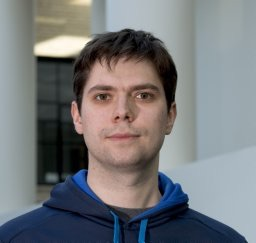
\includegraphics[height=3cm]{../people/vlad}
	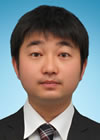
\includegraphics[height=3cm]{../people/yuki}
	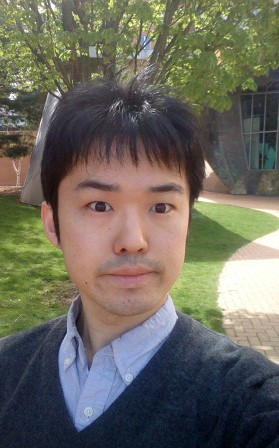
\includegraphics[height=3cm]{../people/hiroki}
	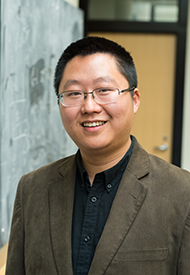
\includegraphics[height=3cm]{../people/liangfu}
\end{center}
\item Working in progress.
\end{itemize}
\end{frame}

\begin{frame}{Outline}
	%\begin{columns}
	%\column{.7\textwidth}
		\tableofcontents
  %\end{columns}
  % You might wish to add the option [pausesections]
\end{frame}

\section{Introduction: Two-Lifetime Models and Fermi Arcs}

\begin{frame}
\frametitle{Two-Lifetime models}
\begin{itemize}
\item Consider a two-band model,
\[H_0=\sum_k\begin{pmatrix}f_{k\alpha}^\dagger&c_{k\alpha}^\dagger\end{pmatrix}
\begin{pmatrix}\epsilon_{fk} & V_k\\ V_k & \epsilon_{ck}\end{pmatrix}
\begin{pmatrix}f_{k\alpha}\\c_{k\alpha}\end{pmatrix}.\]
\item With two lifetimes,
\[G^{-1}(k,\omega)=\omega-H_0(k)-\Sigma_k,\quad
\Sigma_k=-i\begin{pmatrix}\Gamma_f & 0\\0 & \Gamma_c\end{pmatrix}.\]
\item Non-Hermition effective Hamiltonian,
\[H = H_0+\Sigma = \begin{pmatrix}
\epsilon_{fk} - i\Gamma_f & V_k\\ V_k & \epsilon_{ck} - i\Gamma_c
\end{pmatrix}, \quad G=(\omega-H)^{-1}.\]
\end{itemize}
Vlad Kozii and Liang Fu, arXiv:1708.05841.
\end{frame}

\begin{frame}
\frametitle{Exceptional points and Fermi arcs}
\begin{itemize}
\item The non-Hermitian effective Hamiltonian $H = H_0+\Sigma = \begin{pmatrix}
\epsilon_{fk} - i\Gamma_f & V_k\\ V_k & \epsilon_{ck} - i\Gamma_c
\end{pmatrix}$ has {\color{blue}exceptional points} @ $\epsilon_{ck}=\epsilon_{fk}$ \&
$|V_k|=|\Gamma_f-\Gamma_c|$.
\item Electron spectrum density
\[A(k, \omega)=-\frac1\pi\tr\im G(k, \omega)
=-\frac2\pi\im\left(
\frac1{\omega-E_1}+\frac1{\omega-E_2}\right)
=\frac2\pi\sum_{a=1,2}\frac{\im E_a}{(\omega-\re E_a)^2+\im E_a^2}.\]
\end{itemize}

\begin{columns}
\column{.65\textwidth}
\begin{itemize}
\item Along $\epsilon_{ck}=\epsilon_{fk}=\mu$:
\item $|V_k|>|\Gamma_f-\Gamma_c|$: $\re E_1\neq\re E_2$, two peaks, gap open.
\item $|V_k|<|\Gamma_f-\Gamma_c|$: $\re E_1=\re E_2$, one peak, gap close.
\item With $k$-dependence in $V_k$ or $Gamma$ (or both), gap is open/close on part of the Fermi surface: \\{\color{blue}Fermi arcs}.
\item Two ingredients: $V_k\neq0$ and $\Gamma_c\neq\Gamma_f$.
\end{itemize}
\column{.5\textwidth}
%\begin{center}
	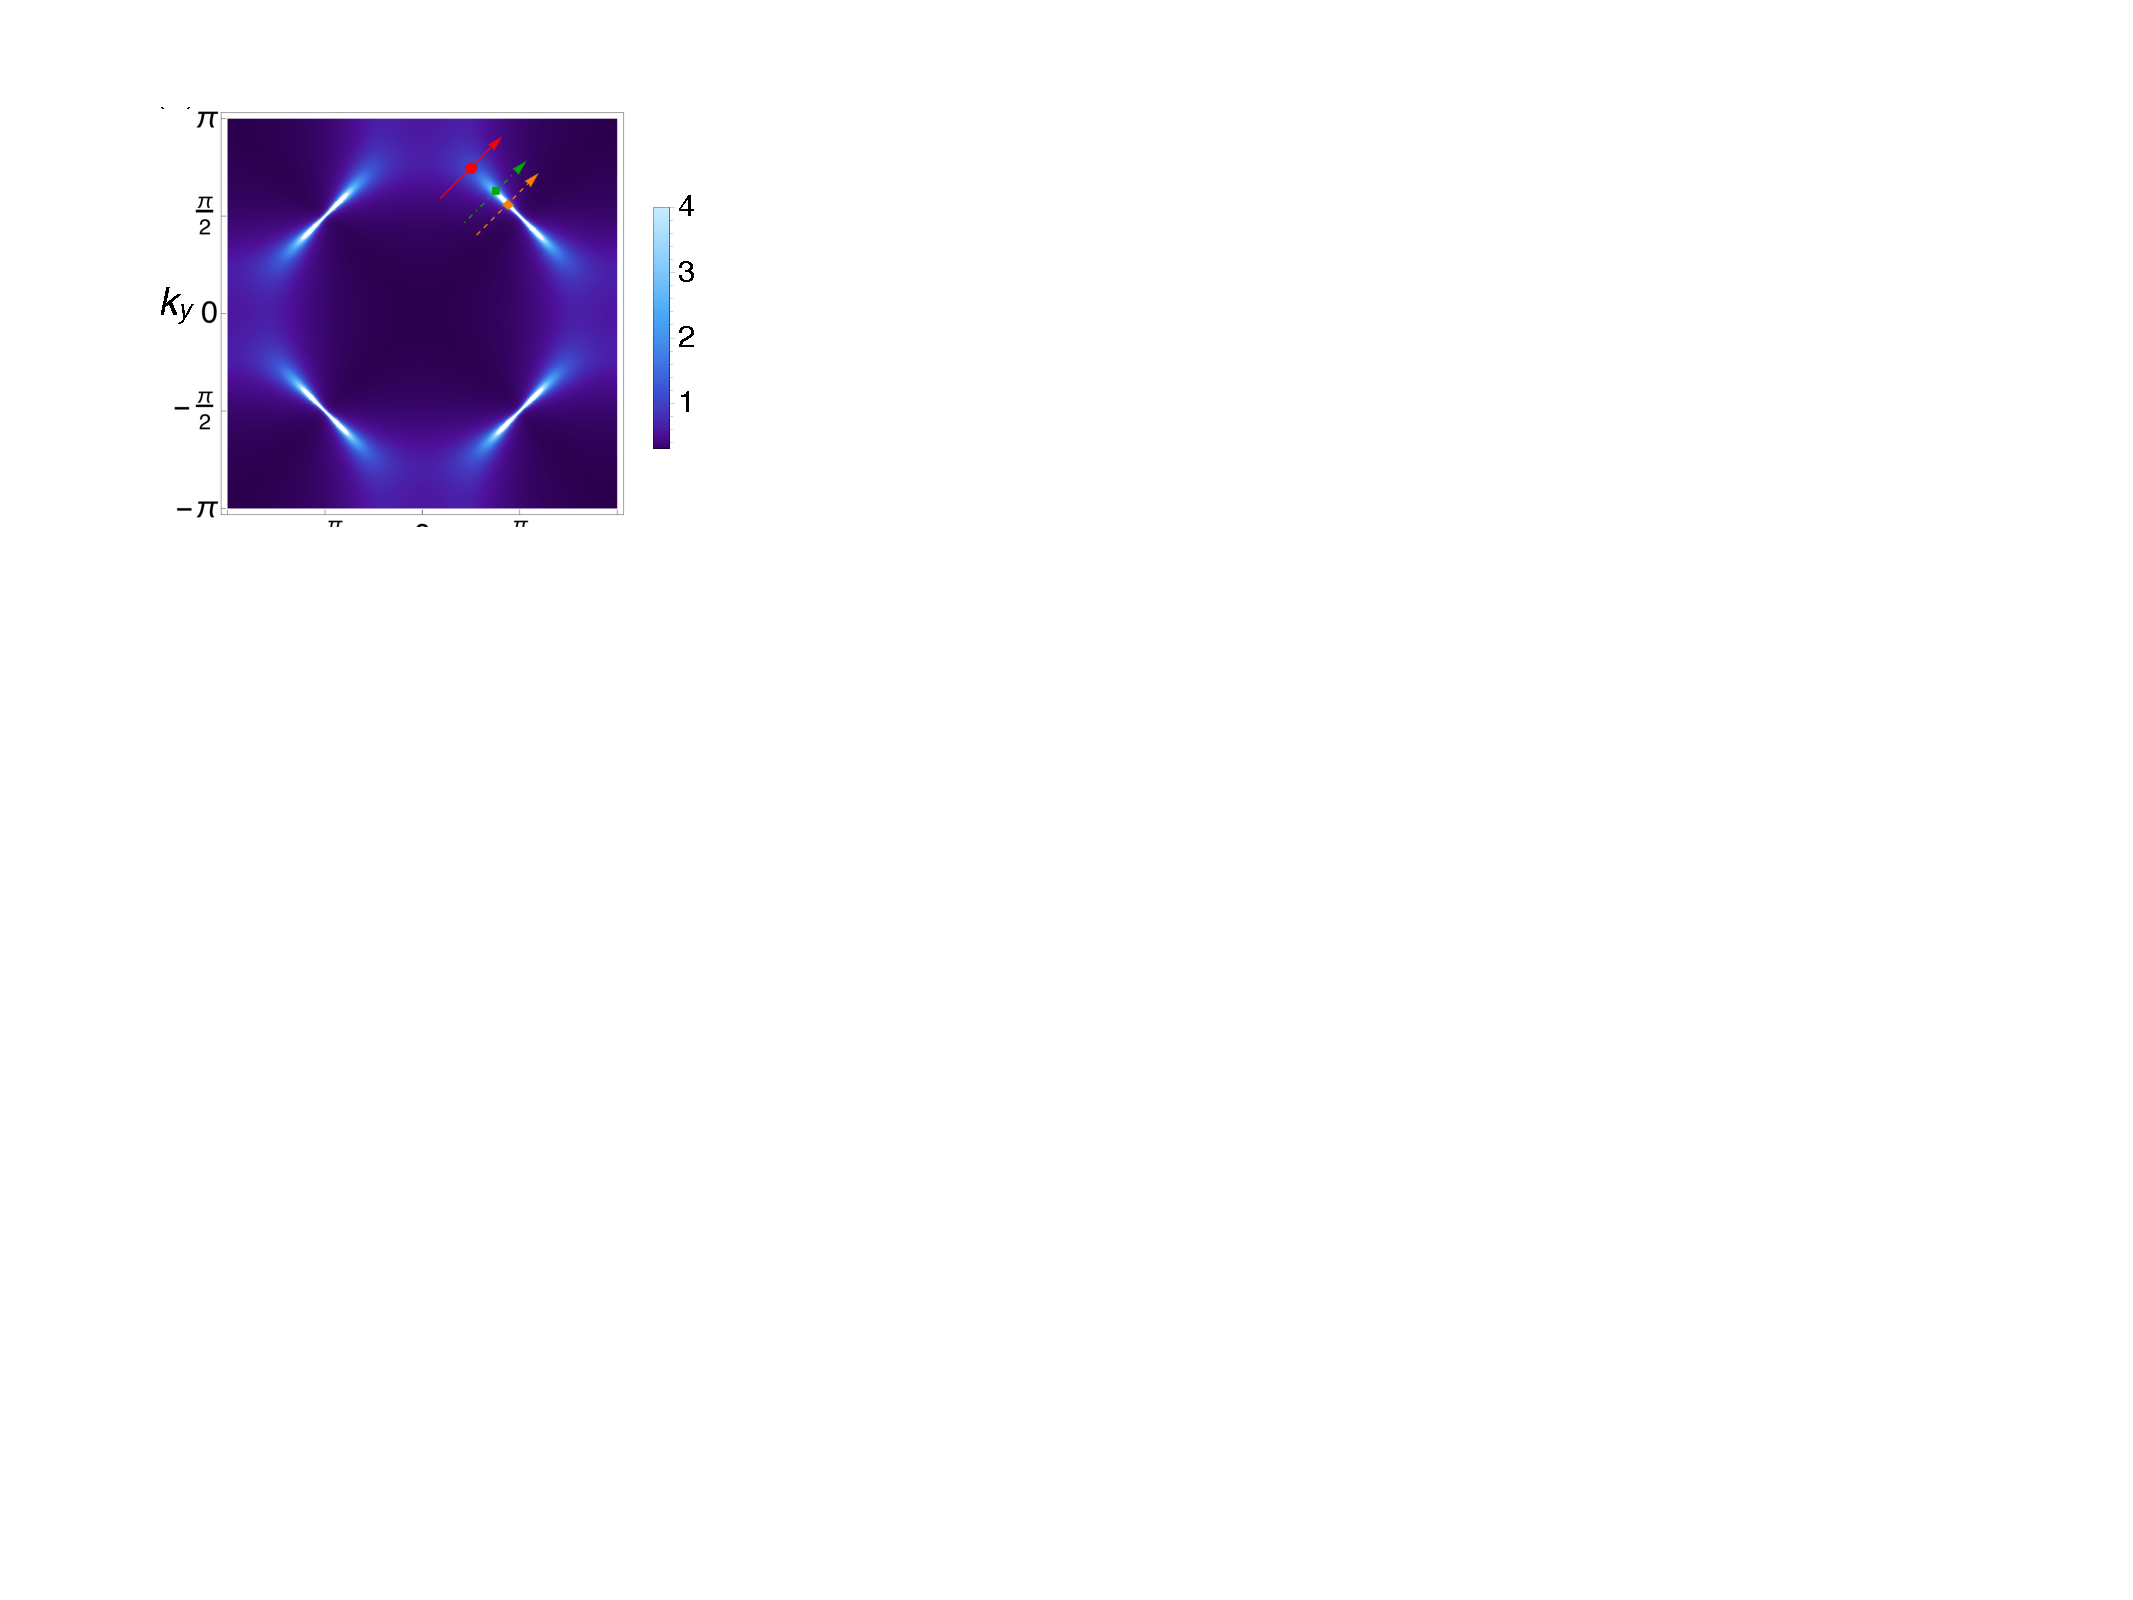
\includegraphics[height=2.5cm]{arc1}
	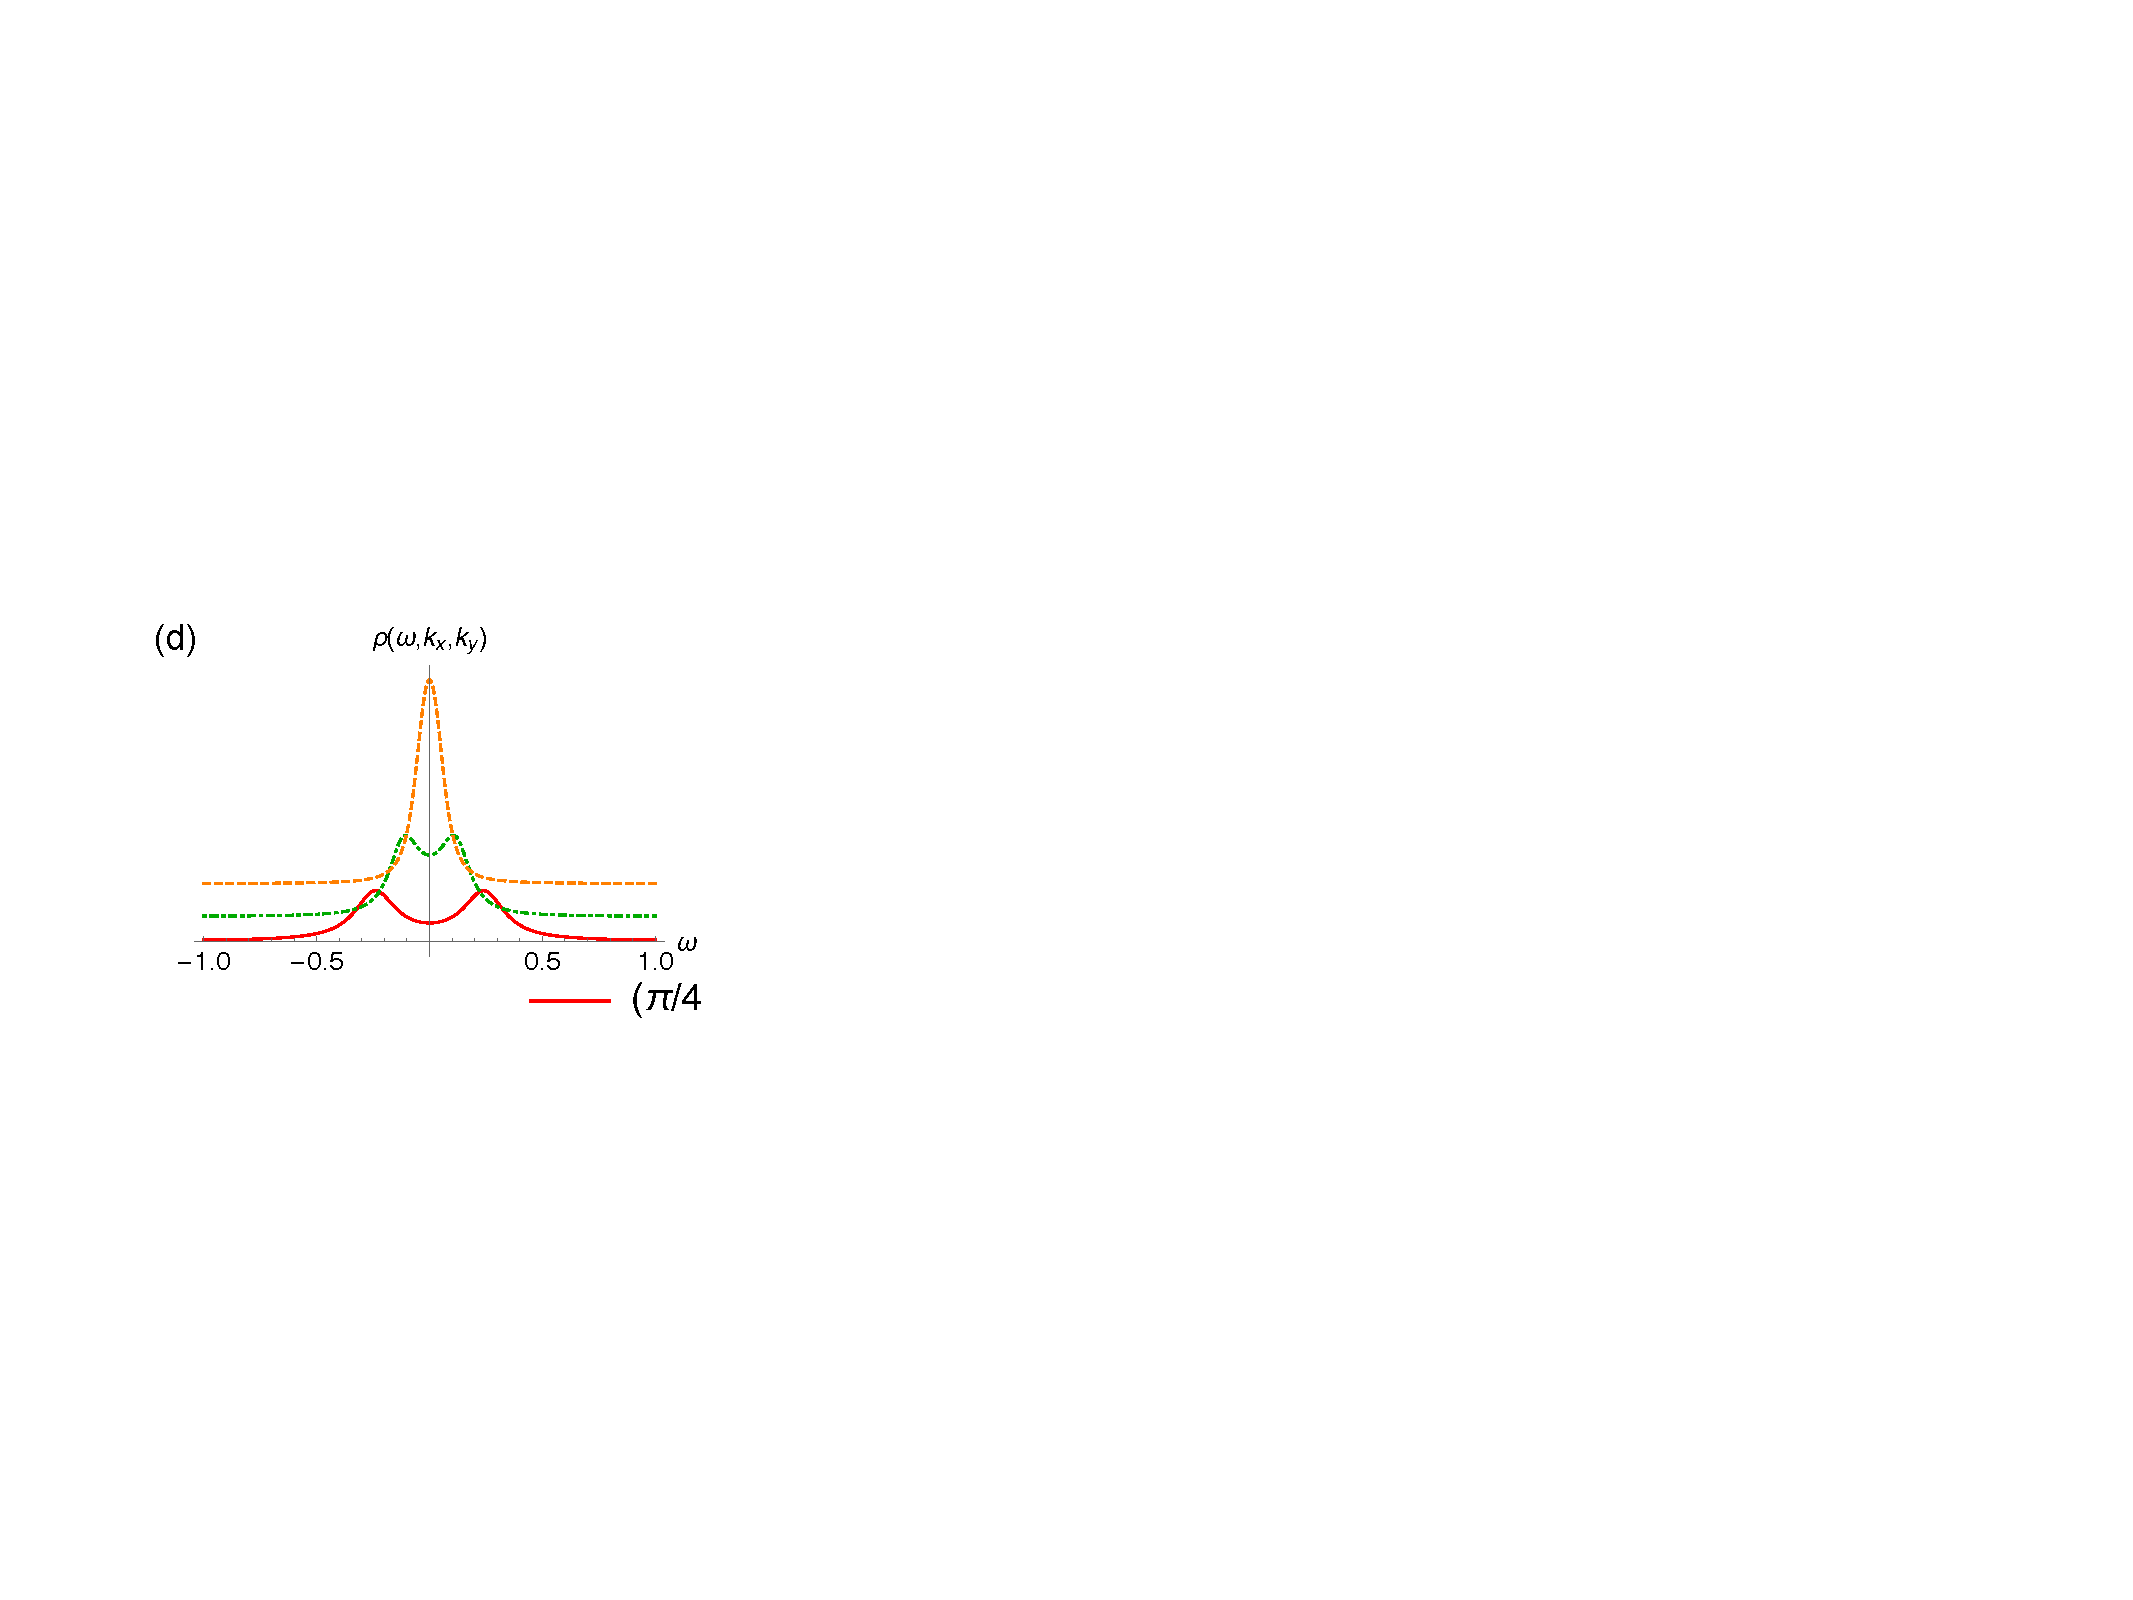
\includegraphics[height=2.5cm]{arc2}
%\end{center}
\end{columns}
\end{frame}

\section{Two Lifetimes and Fermi Arcs in an Anderson-Lattice Model}

\begin{frame}
\frametitle{Anderson-Lattice Model}
\[H=\sum_k\begin{pmatrix}f_{k\alpha}^\dagger&c_{k\alpha}^\dagger\end{pmatrix}
\begin{pmatrix}\epsilon_{fk} & V_k\\ V_k & \epsilon_{ck}\end{pmatrix}
\begin{pmatrix}f_{k\alpha}\\c_{k\alpha}\end{pmatrix}
+U\sum_in_f(n_f-1).\]
\begin{itemize}
\item $f/c$-electron: $\epsilon_{f,c}=-2t_{f,c}(\cos k_x+\cos k_y)$, $t_f\ll t_c$.
\item $d$-wave hybridization: $V_k=v_0(\cos k_x-\cos k_y)$.
\item $u$ interaction: only for the $f$-electron.
\end{itemize}
\end{frame}

\begin{frame}
\frametitle{Two lifetimes due to inelastic scatterings}
\begin{itemize}
\item Consider a series expansion in $u$:
\[
\Sigma = \begin{tikzpicture}[scale=.5]
  %\draw [white] (0, -.1)--(0, 2.2);
  \draw [fermion] (-2, 0) -- (0, 0)
    node [midway, below] {$k$};
  \draw [fermion] (0, 0) -- (2, 0)
    node [midway, below] {$k$};
  \draw [fermion2] (0, 0) to [out = 150, in = 180] (0,2)
    to [out = 0, in = 30] (0, 0);
  \node at (0, 2) [above] {$p$};
  \node at (0, 0) [circle, fill, inner sep=2pt] {};
\end{tikzpicture}
+
\begin{tikzpicture}[scale=.5]
  %\draw [white] (0, -.1)--(0, 2.2);
  \draw [fermion] (-2, 0) -- (0, 0)
    node [midway, below] {$k$};
  \draw [fermion] (0, 0) -- (2, 0)
    node [midway, below] {$k+q$};
  \draw [fermion] (2, 0) -- (4, 0)
    node [midway, below] {$k$};
  \draw [fermion] (0, 0) to [out = 90, in = 180] (1, 1)
    to [out = 0, in = 90] (2, 0);
  \node at (1, 1) [above] {$p$};
  \draw [fermion] (2, 0) to [out = -90, in = 0] (1, -1)
    to [out = 180, in = -90] (0, 0);
  \node at (1, -1) [below] {$p+q$};
  \node at (0, 0) [circle, fill, inner sep=2pt] {};
  \node at (2, 0) [circle, fill, inner sep=2pt] {};
\end{tikzpicture}
+\begin{tikzpicture}[scale=.5]
  %\draw [white] (0, -.1)--(0, 2.2);
  \draw [fermion] (-1, 0) -- (0, 0);
  \draw [fermion] (0, 0) to [out=90, in=180] (1, 1);
  \draw [fermion] (1, 0) -- (0, 0);
  \draw [fermion] (0, 0) to [out=-90, in=180] (1, -1);
  \fill [draw, thick, fill=black!30] (1, 1.2) rectangle (2, -1.2);
  \draw [fermion] (2, 1) to [out=0, in=90] (3, 0);
  \draw [fermion] (3, 0) -- (2, 0);
  \draw [fermion] (2, -1) to [out=0, in=-90] (3, 0);
  \node at (0, 0) [circle, fill, inner sep=2pt] {};
  \node at (3, 0) [circle, fill, inner sep=2pt] {};
  \draw [fermion] (3, 0) -- (4, 0);
\end{tikzpicture}
\]
\item $\Sigma=\begin{pmatrix}\Sigma_f & 0\\ 0 & 0\end{pmatrix}$ to {\color{blue}all orders} of perturbations.
\item Two lifetimes: $\Gamma_f\neq \Gamma_c=0$.
\end{itemize}
\end{frame}
\begin{frame}
\frametitle{2nd-order Perturbation Theory}
\[
\begin{tikzpicture}[scale=.5]
  %\draw [white] (0, -.1)--(0, 2.2);
  \draw [fermion] (-2, 0) -- (0, 0)
    node [midway, below] {$k$};
  \draw [fermion] (0, 0) -- (2, 0)
    node [midway, below] {$k+q$};
  \draw [fermion] (2, 0) -- (4, 0)
    node [midway, below] {$k$};
  \draw [fermion] (0, 0) to [out = 90, in = 180] (1, 1)
    to [out = 0, in = 90] (2, 0);
  \node at (1, 1) [above] {$p$};
  \draw [fermion] (2, 0) to [out = -90, in = 0] (1, -1)
    to [out = 180, in = -90] (0, 0);
  \node at (1, -1) [below] {$p+q$};
  \node at (0, 0) [circle, fill, inner sep=2pt] {};
  \node at (2, 0) [circle, fill, inner sep=2pt] {};
\end{tikzpicture}
\]
\begin{align*}\Gamma_f(k,\omega)&=u^2\int d\omega_{1,2,3}d^2k_{1,2,3}\delta(k-k_1-k_2-k_3)\delta(\omega-\omega_1-\omega_2-\omega_3)\\
&\rho_f(k_1,\omega_1)\rho_f(k_2,\omega_2)\rho_f(k_3,\omega_3)
[n_F(\omega_1)n_F(\omega_2)n_F(-\omega_3)+
n_F(-\omega_1)n_F(-\omega_2)n_F(\omega_3)]
.\end{align*}
\begin{itemize}
\item $T\gg v_0\gg t_f$: $\rho_f$ is $k$-independent $\Rightarrow$ $\Gamma_f$ is also $k$-independent.
\item $\omega$-dependence don't have qualitative effects.
\end{itemize}
\end{frame}

\begin{frame}
\frametitle{Results of the 2nd-Order Perturbation Theory}
\begin{itemize}
\item The $k$-dependence is very weak:
\item Ignoring the $k$-dependence: use the local density of state.
\item Expansion near small $\omega$:
\[\Sigma(\omega) = -ia_0-a_1\omega-ia_2\omega^2,\quad
a_{1,2,3}>0.\]
\item $A(\omega)$ still has one/two peak(s): no qualitative change.
\end{itemize}
\begin{center}
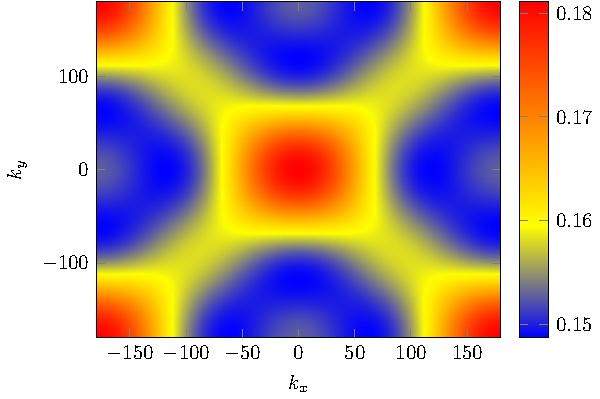
\includegraphics[height=3.5cm]{gammak_v1}
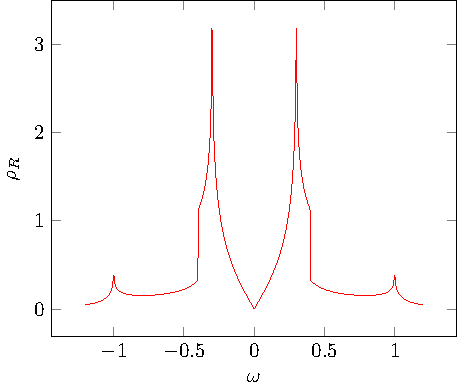
\includegraphics[height=3.5cm]{rho_dwave0}
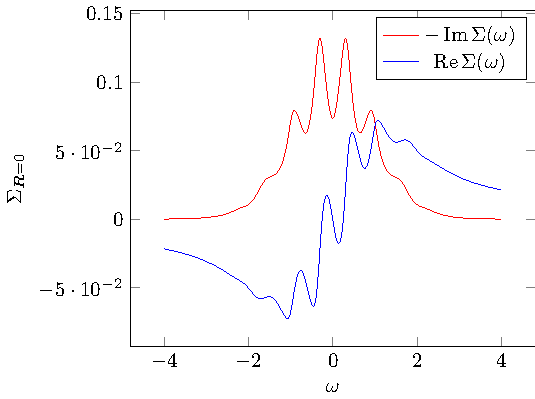
\includegraphics[height=3.5cm]{ims_dwave}
\end{center}
\end{frame}

\begin{frame}
\frametitle{Summary}
\begin{itemize}
\item<1-7> An Anderson-Lattice model w/ d-wave hybridization.
\item<2-5> We computed electron self energy using second-order perturbation theory.
\item<3-8> $\Gamma_f\neq\Gamma_c=0$.
\item<4-6> At $T\geq v_0$, $\Sigma_f$ can be treated as a constant.
\item<5-9> $\Gamma_f\neq\Gamma_c$ and a $k$-dependent $V_k$ results in Fermi arcs:
\begin{enumerate}
\item $V_k<\Gamma_f$: one peak = Fermi arc. Like a small Fermi surface.
\item $V_k>\Gamma_f$: two peaks = gapped. Like a Kondo insulator.
\item A dichotomy on the Fermi surface.
\end{enumerate}
\end{itemize}
\begin{center}
	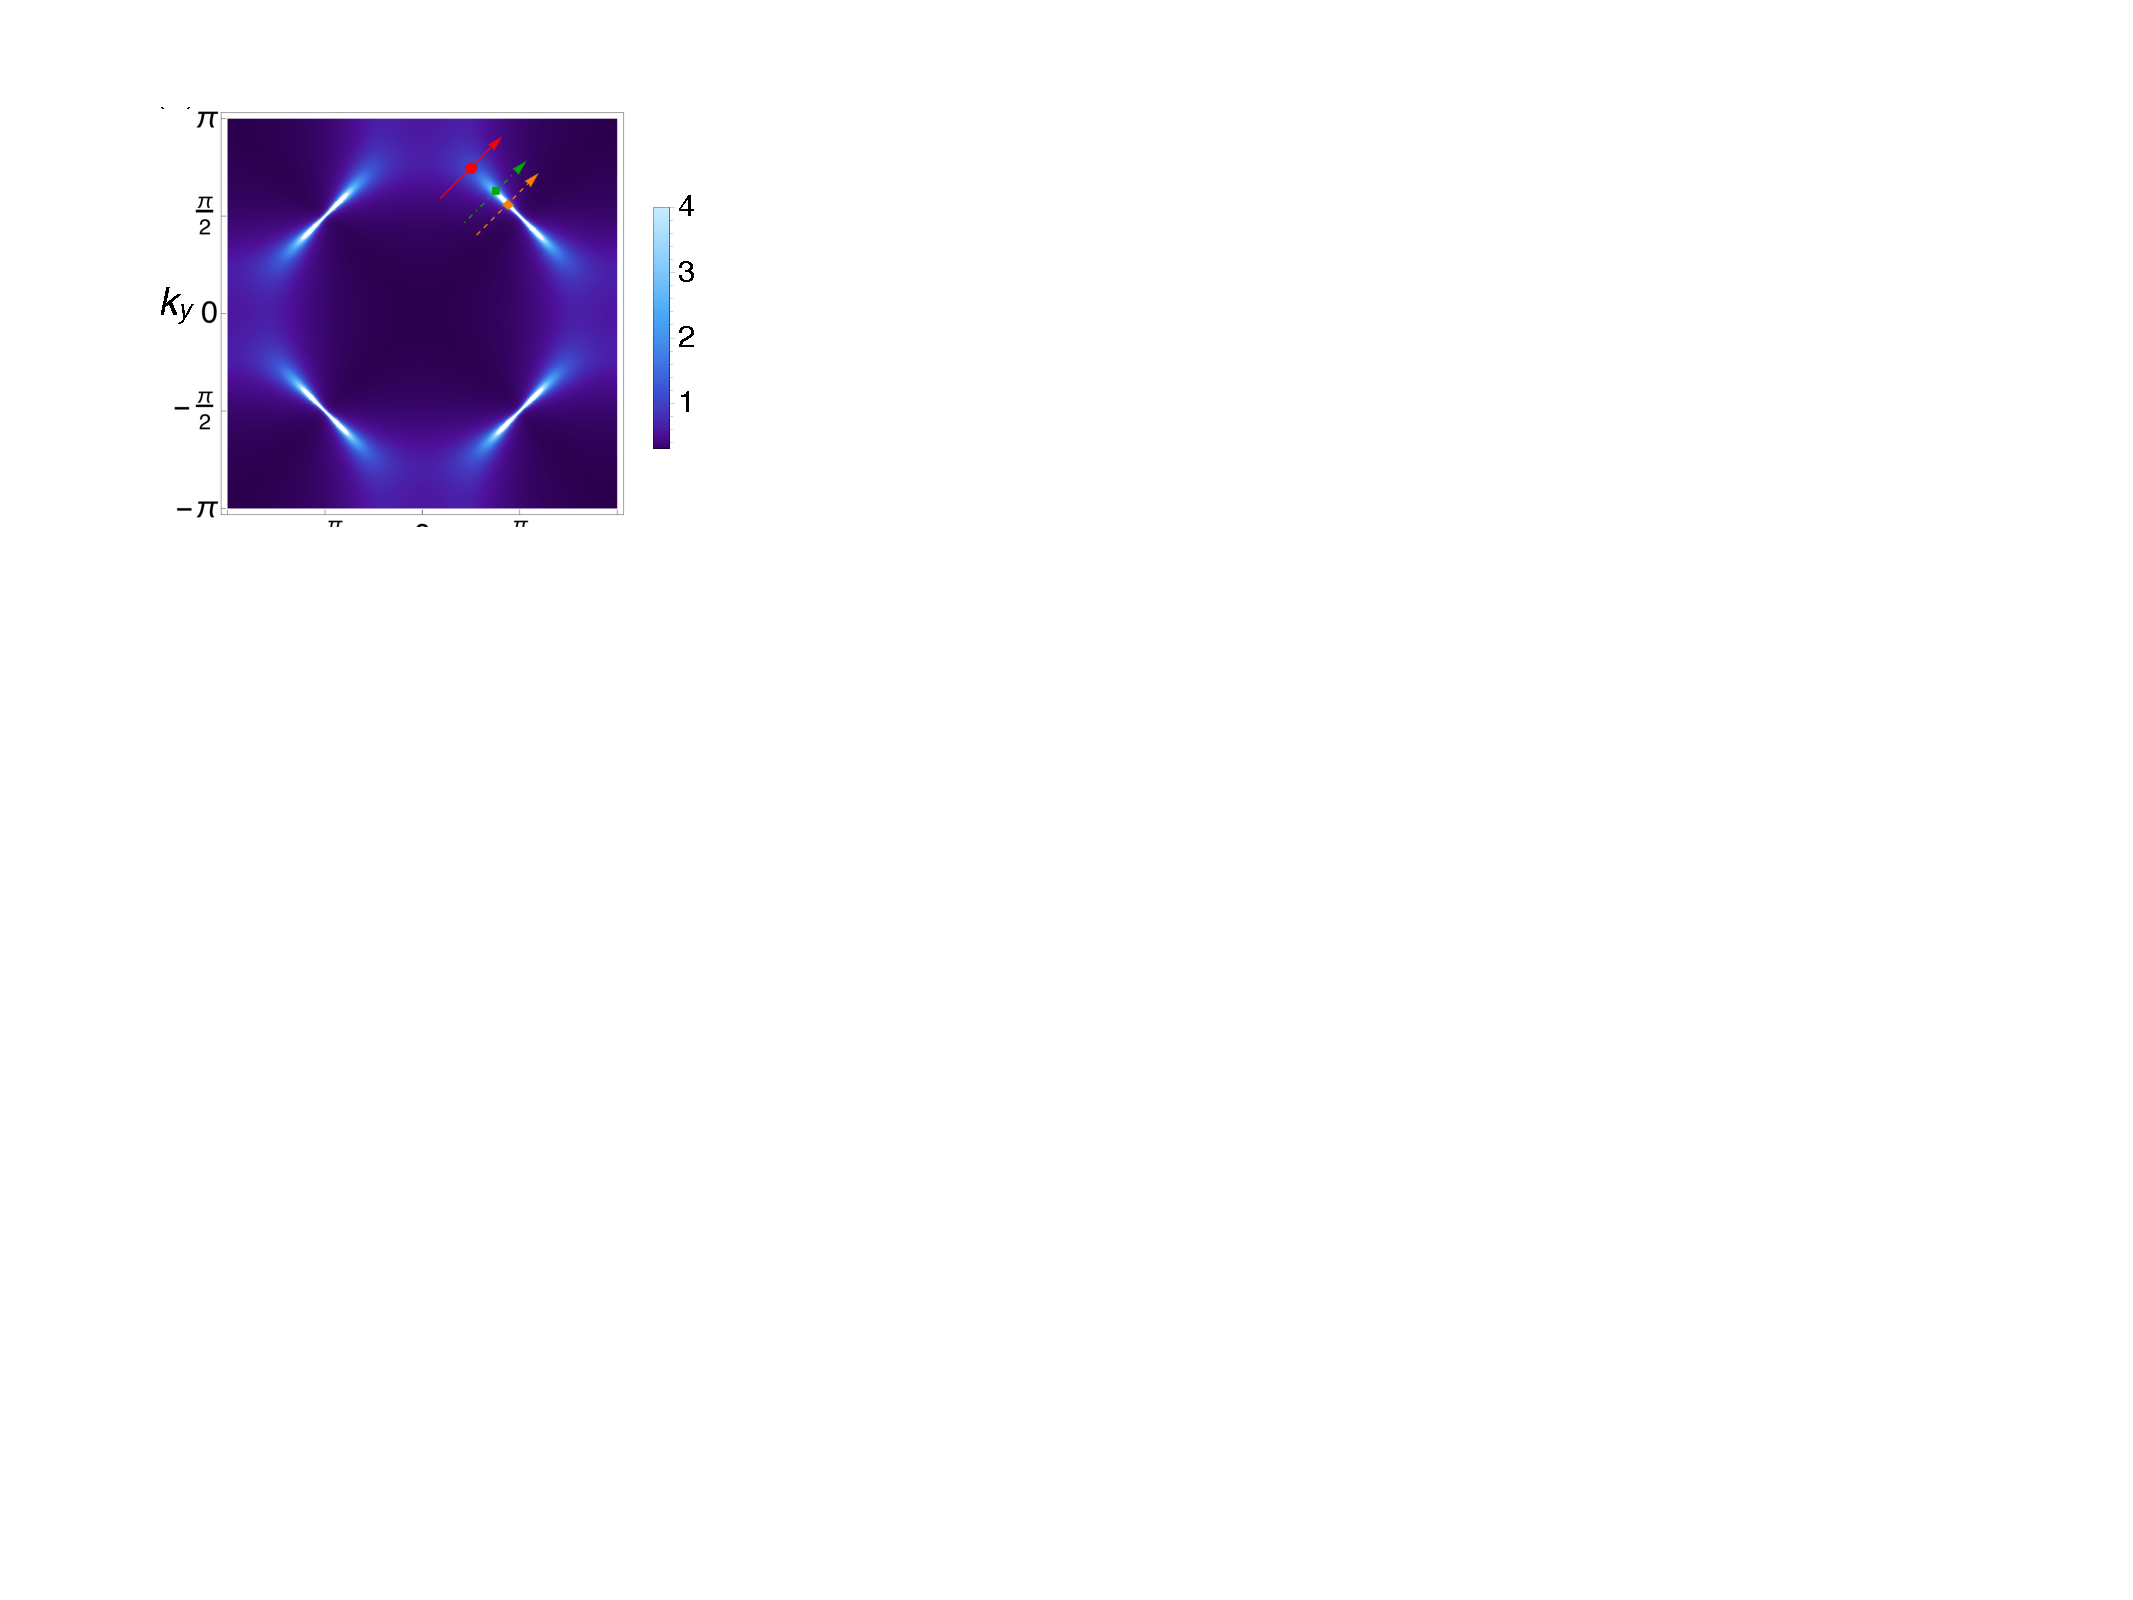
\includegraphics[height=3cm]{arc1}~~~~
	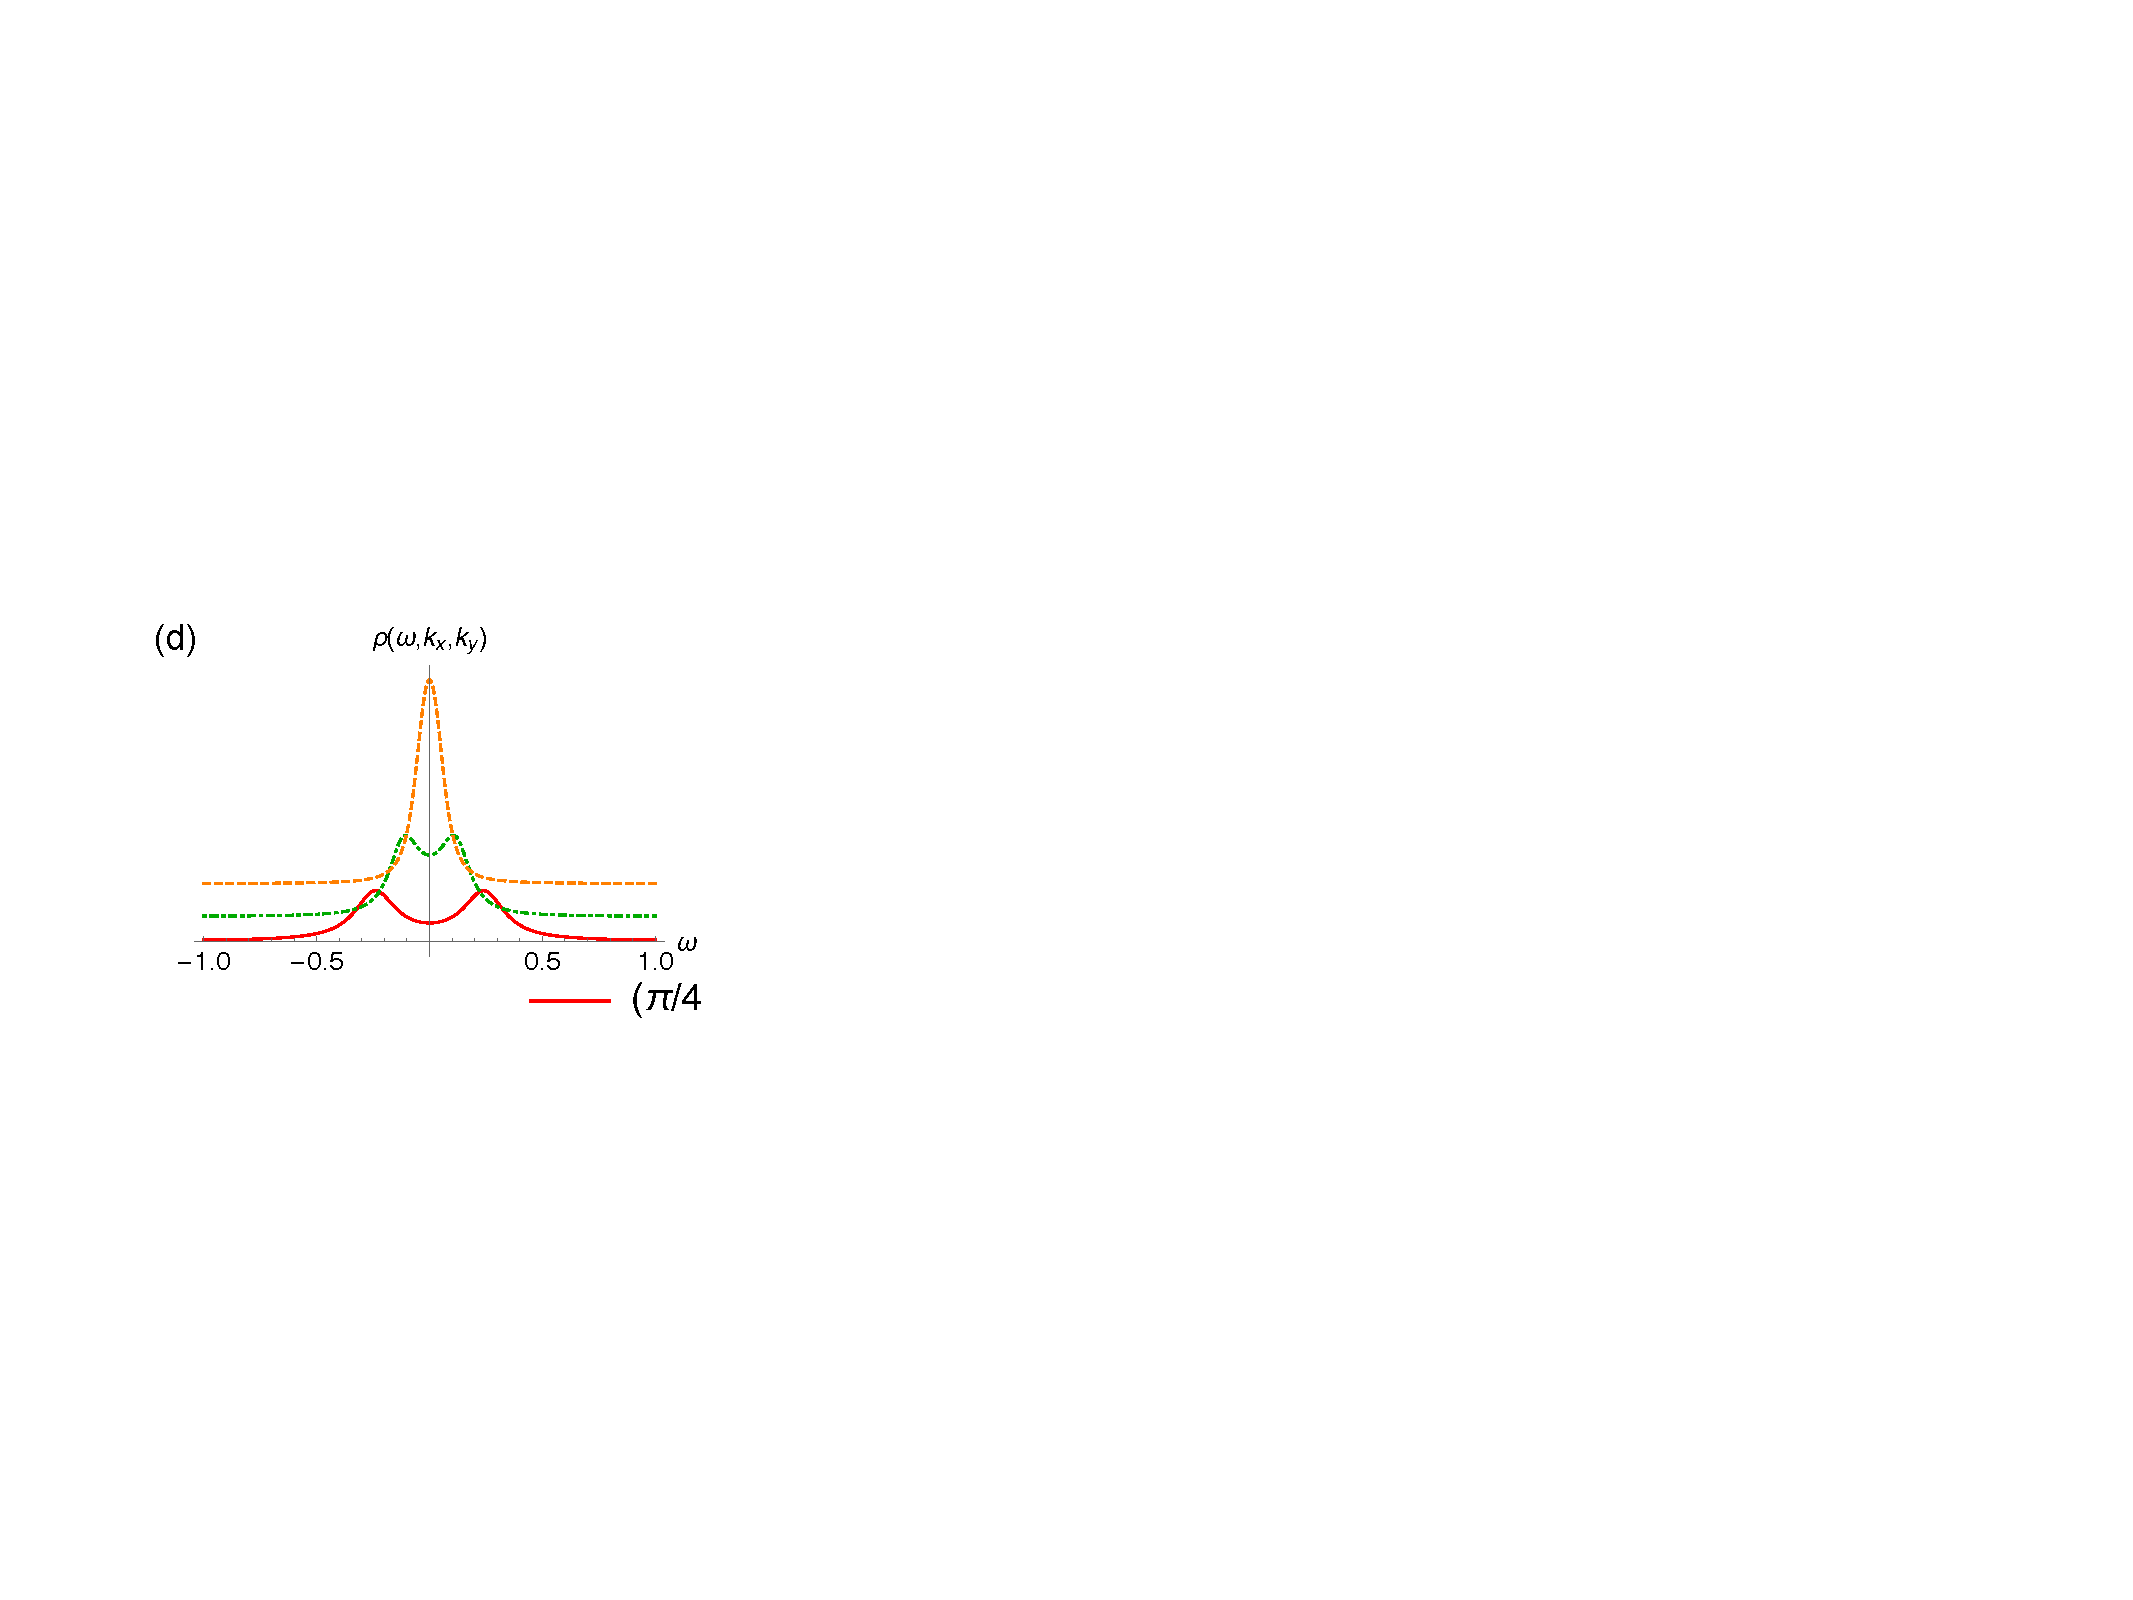
\includegraphics[height=3cm]{arc2}
\end{center}
\end{frame}

%\section{Fermi Arcs}

%\section{Conclusion}

\end{document}
